\section{Energy Measurement Setup}

\subsection{Instrumentation and Procedure}
\textbf{ESP32 and Raspberry Pi:} current and voltage were sampled every 500 ms using INA219. Two windows were captured: idle ($N_{idle}$ samples) and load ($N_{load}$ samples) during benchmark execution.\newline
\textbf{Android devices:} current and voltage were read from system APIs under controlled idle/load phases.
The complete instrumentation and sampling windows are summarized in Table~\ref{tab:energy_setup}.

Incremental power was estimated as
\begin{equation}
\Delta P = P_{load} - P_{idle},
\end{equation}
and energy per inference as
\begin{equation}
E_{inf} = \frac{\Delta P}{\text{throughput}}.
\end{equation}

\begin{table}[t]
\caption{Measured setup and sampling windows by platform.}
\label{tab:energy_setup}
\centering
\begin{tabular}{lccc}
\toprule
Platform & Sensor/Source & Idle samples & Load samples \\
\midrule
ESP32 (MicroPython) & INA219 & 50 & 50 \\
Raspberry Pi 4B & INA219 & 97 & 440 \\
Android (A/B/C) & System telemetry & 200 & 200 \\
\bottomrule
\end{tabular}
\end{table}


Figure~\ref{fig:speed_energy_setup} summarizes the deployment envelope by combining throughput and incremental energy per inference in a single view. Movement to the right indicates faster processing, while downward movement indicates lower energy cost per prediction. This representation highlights that the best operating point depends on application cadence: high-rate scenarios favor smartphone and SBC execution, whereas low-rate autonomous sensing can still be supported on microcontroller-class hardware.


\begin{figure}[t]
\centering
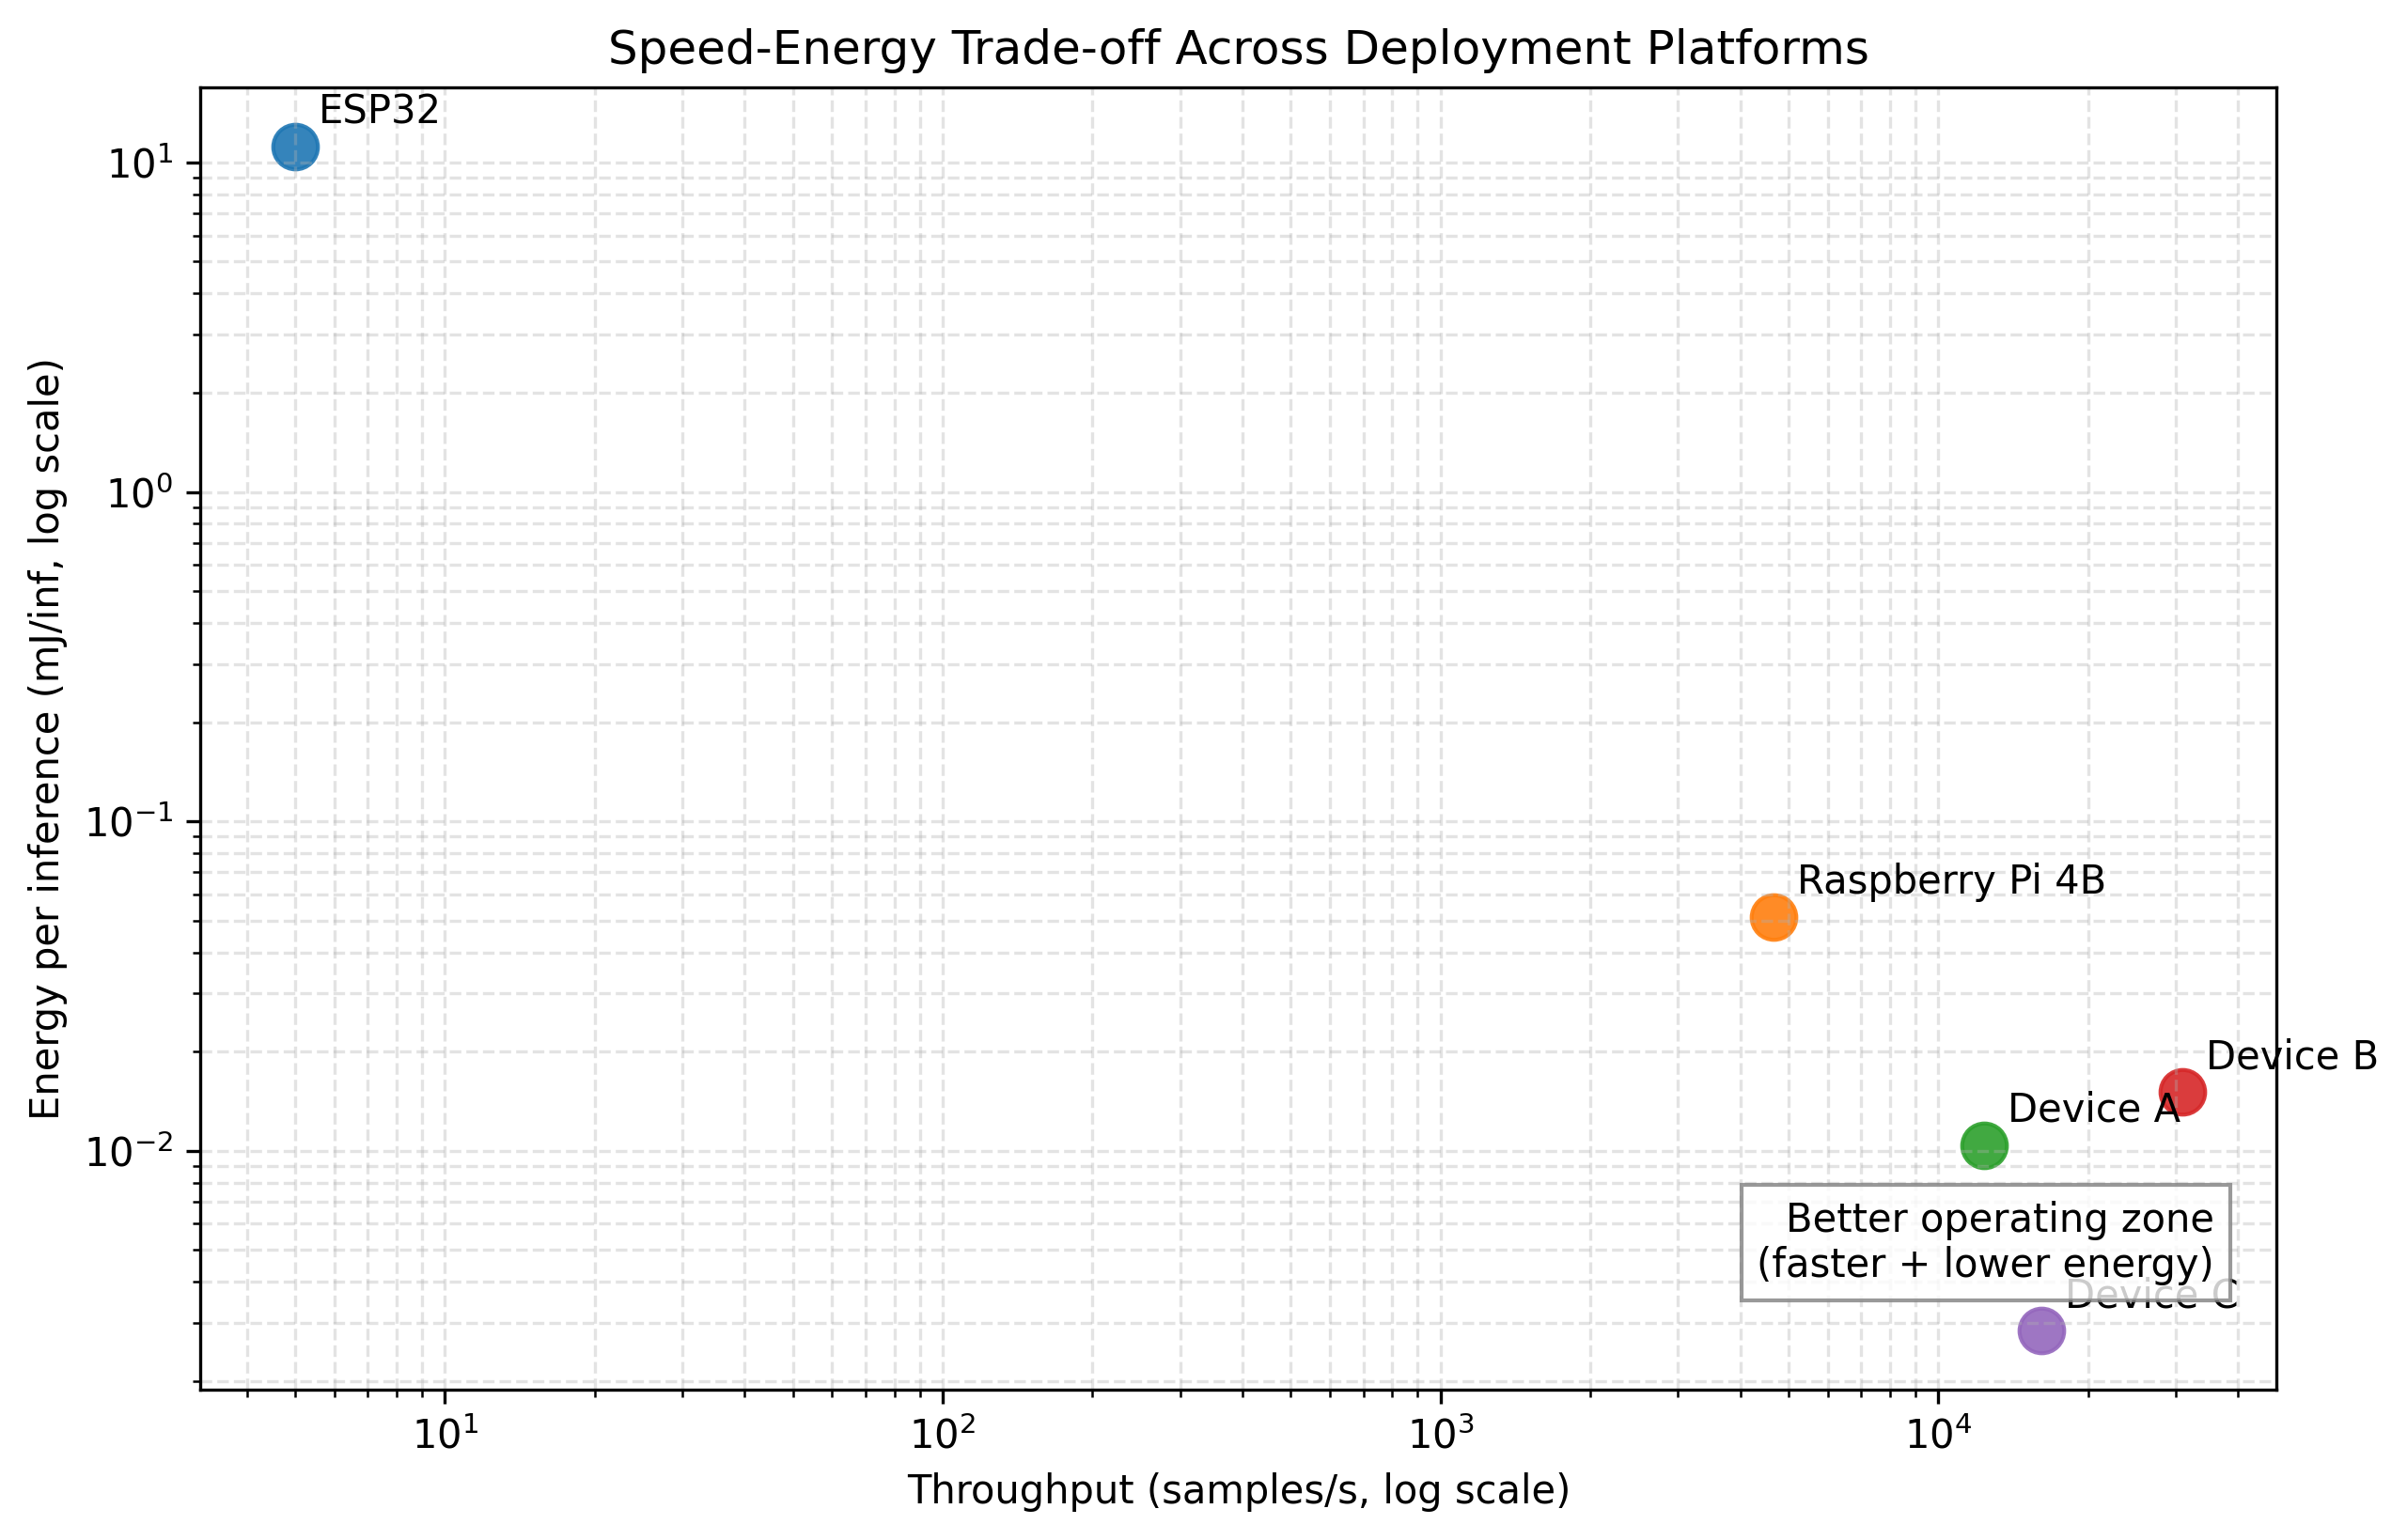
\includegraphics[width=0.88\textwidth]{speed_energy_tradeoff.png}
\caption{Speed--energy positioning of evaluated platforms (log scales).}
\label{fig:speed_energy_setup}
\end{figure}
